
\section{Methodology}
\label{sec:method}

Given the focus on periodicity, we adopt the channel-independent paradigm~\citep{nie2023patchtst, zeng2023dlinear} and omit the channel dimension throughout the remainder of this paper\blue{; the $C$ channels of a dataset share one model}. The objective of forecasting is to predict the future trajectory $\mathbf{Y}\in\mathbb{R}^{L_{\text{out}}}$ from an input sequence $\mathbf{X}\in\mathbb{R}^{L_{\text{in}}}$, where $L_{\text{in}}$ and $L_{\text{out}}$ denote the input and output lengths, respectively. In the following sections, we describe the data preprocessing procedure, present the proposed network architecture \blue{and the scope of its phase alignment, introduce its level--amplitude extension, and finally analyze the computational complexity of both}.

\begin{figure*}[t]
    \centering
    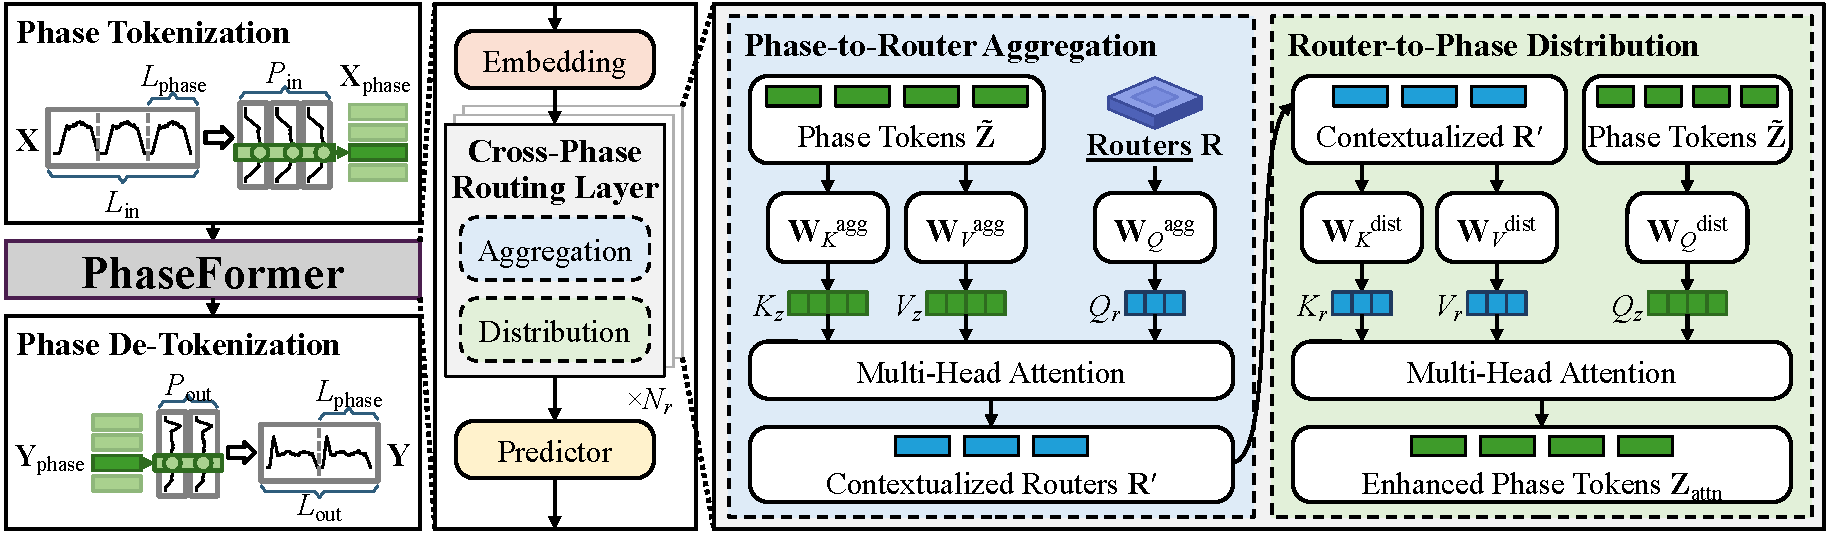
\includegraphics[width=\textwidth]{figures/phaseformer_overview.pdf}
    \caption{\blue{Overview} of \sysname.}
    \label{fig:overview}
\end{figure*}

\subsection{Data \blue{Preprocessing}}
\label{subsec:phase-embedding}
\fakeparagraph{Normalization and De-Normalization}
Following \cite{kim2021reversible}, we normalize inputs with their estimated mean and standard deviation, and de-normalize predictions to the original scale. \blue{This normalization (RevIN) maps an input window $x$ with mean $\mu$ and standard deviation $\sigma$ to $\tilde x=(x-\mu\one)/\sigma$, so that $\one^\top\tilde x=0$, and a forecast $\hat{\tilde y}$ in these coordinates is de-normalized to $\hat y=\mu\one+\sigma\hat{\tilde y}$.}

\fakeparagraph{Phase Tokenization and De-Tokenization}
Phase tokenization transforms the one-dimensional input sequence into a two-dimensional phase--period matrix for \blue{subsequent} processing.
Conversely, phase de-tokenization reconstructs the predicted phase--period matrix back into a one-dimensional output sequence.
\revised{\blue{Let $L_{\text{phase}}$ denote the period length; it is estimated by frequency analysis (\secref{sec:phase_length}) and kept fixed.}}

To ensure that the input sequence length is a multiple of $L_{\text{phase}}$, we circularly pad the sequence to length \blue{$P_{\text{in}}L_{\text{phase}}$}, where $P_{\text{in}} = \left\lceil \frac{L_{\text{in}}}{L_{\text{phase}}} \right\rceil.$
As illustrated in \figref{fig:overview}, the padded sequence $\mathbf{X}$ is then reshaped into a phase--period matrix $\mathbf{X}_{\text{phase}} \in \mathbb{R}^{L_{\text{phase}} \times P_{\text{in}}}$, where each entry \blue{$\mathbf{X}_{\text{phase}}[p, k]$ corresponds to the observation at the $p$-th phase of the $k$-th cycle}.
\blue{De-tokenization reverses this reshaping.}

\blue{
\fakeparagraph{Notation}
We abbreviate $P=\Lp$ for the period, $K=\Pin$ and $K'=\Pout$ for the numbers of input and output cycles, $L=KP$ and $H=K'P$. In all \sysLA experiments $L=720$, $P=24$ and $K=30$, and every horizon $H\in\{96,192,336,720\}$ is a whole number of cycles, so that no padding occurs. The folded normalized window $\tilde X\in\mathbb R^{K\times P}$, the transpose of the phase--period matrix of $\tilde x$, has one row per cycle as in Section~\ref{sec:mot_changes}; its columns are the phase tokens $\tilde x_p\in\mathbb R^K$, and its row means are the cycle means $\bar r=\tfrac1P\tilde X\one_P\in\mathbb R^K$.
}

% --------------------------------------------------------------------
\subsection{Phase-\blue{Based} Routing Transformer}
\label{subsec:phase-network}

The phase--period matrix is fed into our proposed phase-based routing Transformer, termed \sysname, to capture and extrapolate temporal dynamics at the phase level.
As illustrated in \figref{fig:overview}, \sysname first applies an embedding layer to the phase tokens, then refines them through multiple cross-phase routing layers, and finally maps them to the target via a shared predictor.

% ---------------- embedding ----------------
\subsubsection{Embedding Layer}
\label{subsubsec:phase-embedding}
The embedding layer projects the phase tokens $\mathbf{X}_{\text{phase}}$ into a low-dimensional representation space, allowing the informative components to be extracted from raw observations that are often contaminated by perturbations.
Formally, for each phase index \blue{$p \in \{1,\dots,L_{\text{phase}}\}$, the corresponding phase token $\mathbf{X}_{\text{phase}}[p, :]$} is mapped into a $d$-dimensional representation through \blue{an affine map $f_{\theta}$ with weight $W_e\in\mathbb R^{d\times\Pin}$ and bias $c_e\in\mathbb R^d$, followed by a LayerNorm $\LN_e$~\citep{ba2016layernorm}}:
\begin{equation}
\mathbf{Z}
= \blue{\LN_e\big(}f_{\theta}\!\left(\mathbf{X}_{\text{phase}}\right)\blue{\big)}\in \mathbb{R}^{L_{\text{phase}}\times d}
\label{eq:phase-embedding}
\end{equation}

To better capture the temporal ordering among phases, we introduce a set of learnable positional embeddings $\mathbf{E}_{\text{pos}}\in\mathbb{R}^{L_{\text{phase}}\times d}$ \blue{to encode the position of each phase within the cycle}, following \cite{liu2023spatio}.
These embeddings are added to $\mathbf{Z}$ in a phase-wise manner, so that each phase representation is enriched with its positional information:
\begin{equation}
\tilde{\mathbf{Z}}=\mathbf{Z}+\mathbf{E}_{\text{pos}}.
\end{equation}
The resulting $\tilde{\mathbf{Z}}$ is then forwarded to the cross-phase routing layers for higher-level feature interaction and forecasting\blue{; in a stack of layers, every layer adds its own positional embeddings to its input in this way}.

% ---------------- Attention ----------------
\subsubsection{Cross-Phase Routing Layer}

Directly modeling full pairwise interactions among phase representations via self-attention is computationally expensive.
To handle this, we introduce a set of learnable routers $\mathbf{R}\in\mathbb{R}^{M\times d}$ to mediate information exchange across phases.
\revised{
While the design is inspired by prior routing-style \blue{designs}~\citep{jaegle2021perceiver, zhang2023crossformer}, our contribution lies in \emph{leveraging the inherent low-rank structure of phase-aligned tokens} \blue{(Insight~2, Section~\ref{sec:mot_stability})}.
\blue{Cross-phase routing reduces the quadratic cost of self-attention to a cost linear in the number of phases, while every phase can still exchange information with every other phase.}
}

Cross-phase routing consists of two steps:
(i) \emph{phase-to-router aggregation}, which selectively compresses information from phase representations into the compact set of routers; and (ii) \emph{router-to-phase distribution}, which selectively propagates the aggregated cross-phase information from the routers back to the phase representations. Both steps are implemented via cross-attention.

\fakeparagraph{Phase-to-Router Aggregation}
The routers attend to the phase representations to extract contextual information, yielding contextualized router embeddings
\blue{$\mathbf{R}'\in\mathbb{R}^{M\times d}$}.
Specifically, the routers act as queries while the phases provide keys and values. The projection matrices
$\mathbf{W}_Q^{\text{agg}},\mathbf{W}_K^{\text{agg}},\mathbf{W}_V^{\text{agg}}\in\mathbb{R}^{d\times d}$
map the representations into query, key, and value spaces, respectively:
\begin{equation}
\mathbf{Q}_r=\mathbf{R}\mathbf{W}_Q^{\text{agg}},\quad
\mathbf{K}_z=\tilde{\mathbf{Z}}\mathbf{W}_K^{\text{agg}},\quad
\mathbf{V}_z=\tilde{\mathbf{Z}}\mathbf{W}_V^{\text{agg}}.
\end{equation}
The aggregated router embeddings are then obtained via multi-head attention (MHA) with \blue{$n_h$} heads:
\begin{equation}
\blue{\mathbf{R}'}=\mathrm{MHA}\!\left(\mathbf{Q}_r,\mathbf{K}_z,\mathbf{V}_z\right).
\end{equation}

\fakeparagraph{Router-to-Phase Distribution}
The aggregated information in the routers is subsequently redistributed to the phase representations, thereby enabling cross-phase information flow. In this step, the phase representations serve as queries while the routers provide keys and values, yielding refined phase representations $\mathbf{Z}_{\text{attn}}$. The projection matrices $\mathbf{W}_Q^{\text{dist}}, \mathbf{W}_K^{\text{dist}}, \mathbf{W}_V^{\text{dist}}\in\mathbb{R}^{d\times d}$ are used for this distribution:
\begin{equation}
\mathbf{Q}_z=\tilde{\mathbf{Z}}\mathbf{W}_Q^{\text{dist}},\quad
\mathbf{K}_r=\blue{\mathbf{R}'}\mathbf{W}_K^{\text{dist}},\quad
\mathbf{V}_r=\blue{\mathbf{R}'}\mathbf{W}_V^{\text{dist}},
\end{equation}
\begin{equation}
\mathbf{Z}_{\text{attn}}=\mathrm{MHA}\!\left(\mathbf{Q}_z,\mathbf{K}_r,\mathbf{V}_r\right).
\end{equation}
This mechanism restores phase-level resolution while simultaneously enforcing coherence across phases through the contextualized routers.
Ultimately, each phase representation attends to all others through a two-stage routing pathway.
\blue{The two steps are wrapped in residual connections, two LayerNorms and an MLP: writing $z_p$ and $m_p$ for the $p$-th rows of the layer input ($\tilde{\mathbf Z}$ for the first layer) and of $\mathbf Z_{\text{attn}}$, a routing layer outputs $o_p=\LN_1(z_p+m_p)$ and $h_p=\LN_2\big(o_p+\mathrm{MLP}(o_p)\big)$. Each LayerNorm centers its input over the $d$ features, rescales it to unit root mean square, and applies a learned gain $\gamma_i$ and offset $\beta_i$: $\LN_i(u)=\gamma_i\odot\varsigma+\beta_i$ with $\varsigma=J_du/(\|J_du\|^2/d+\epsilon)^{1/2}$ and $J_d=I_d-\tfrac1d\one\one^\top$. Hence $\|\varsigma\|<\sqrt d$ for every input, and every latent $h_p$ of the last layer is an output of its $\LN_2$; Section~\ref{sec:theory} builds on these two facts. Appendix~\ref{app:proofs} states the full layer.}


% ---------------- predictor ----------------
\subsubsection{Predictor}
\label{subsubsec:phase-predictor}

The predictor produces multi-step forecasts of length $P_{\text{out}}$ for all phases simultaneously, based on their refined representations. Taking as input the \blue{final phase latents $\mathbf Z_{\text{out}}=[h_1;\dots;h_{L_{\text{phase}}}]\in\mathbb{R}^{L_{\text{phase}}\times d}$ of the last} cross-phase routing layer, the predictor is realized as \blue{an affine} mapping \blue{$g_{\Phi}$}, parameterized by \blue{a weight $\Phi\in\mathbb{R}^{P_{\text{out}}\times d}$ and a bias $c_\Phi\in\mathbb{R}^{P_{\text{out}}}$ and applied to every phase}:
\begin{equation}
\begin{gathered}
\mathbf{Y}_{\text{phase}} = \blue{g_{\Phi}(\mathbf Z_{\text{out}})}
\in \mathbb{R}^{L_{\text{phase}}\times P_{\text{out}}}\blue{,}\\
\blue{F_p=\Phi h_p+c_\Phi\in\mathbb R^{K'}.}
\end{gathered}
\label{eq:predictor}
\end{equation}
\blue{The $p$-th row of $\mathbf Y_{\text{phase}}$ holds the $K'$ future values $F_p$ of phase $p$ in normalized units. Unfolding the phases cycle by cycle gives the \emph{phase forecast} $F\in\mathbb R^H$, and we call the computation from the phase tokens to $F$ the \emph{phase path}; for \sysname, the forecast is $\hat{\tilde y}=F$.}
All phases share the same predictor parameters, which enforces consistency across phases and reduces the number of trainable parameters. This not only improves efficiency but also regularizes learning, thereby enhancing generalization. Finally, the predicted phase--period matrix $\mathbf{Y}_{\text{phase}}$ is passed through de-tokenization and de-normalization to produce the final forecast $\mathbf{Y}$.


\revised{
\subsection{\blue{Scope of Phase Alignment}}
\label{sec:discussion}

\blue{
\fakeparagraph{Weak Periodicity}
Although \sysname is built around periodic alignment, it remains usable on weakly periodic or partially non-periodic time series. When no strong periodic structure is present, the phase representation degenerates into a coarse subsampling of the sequence: the phase tokens resemble trend embeddings sampled every $\Lp$ steps and capture slowly varying components and broad temporal structure. Through the routing mechanism, the model can still aggregate information across these coarse tokens, which suppresses high-frequency noise, prevents overfitting to short-term stochastic fluctuations, and retains a certain degree of robustness without a clear period.

\fakeparagraph{Failure Modes}
In datasets without a clear dominant period, the estimated phase length may be affected by noise or minor harmonics, and the resulting misalignment is the primary failure mode of the model. In multi-period settings, a model aligned to a suboptimal harmonic instead of the dominant component still operates but delivers inferior forecasts (\secref{sec:phase_length}). A phase length that is excessively large or small also introduces substantial circular padding, which injects artificial boundary information and degrades the forecasts; input lengths divisible by the phase length avoid it and are recommended whenever possible.

This subsection concerns series without a reliable period. Within a periodic series, the changes across cycles of Section~\ref{sec:mot_changes} are a different limitation, which the extension below addresses.
}
}


\blue{
\subsection{\sysLA: Supplying the Missing Level and Amplitude}
\label{sec:extension}

\sysname was not designed for the changes across cycles of Section~\ref{sec:mot_changes}. A trained \sysname follows them only within two envelopes fixed by its final LayerNorm and its predictor, one for the level and one for the within-cycle amplitude, and Section~\ref{sec:theory} shows that what lies outside them has a simple form (Table~\ref{tab:two_envelopes}). \sysLA supplies this remainder with two components and keeps the backbone unchanged: phase tokenization, embedding, cross-phase routing and the shared predictor are those of \sysname. A level branch with a gated fusion addresses level drift; we call \sysname with these two parts \sysL. A centered modulation of the final phase latents addresses level-dependent amplitude; adding it to \sysL gives \sysLA. Fig.~\ref{fig:la_overview} shows where the components attach.

\begin{figure*}[t]
\centering
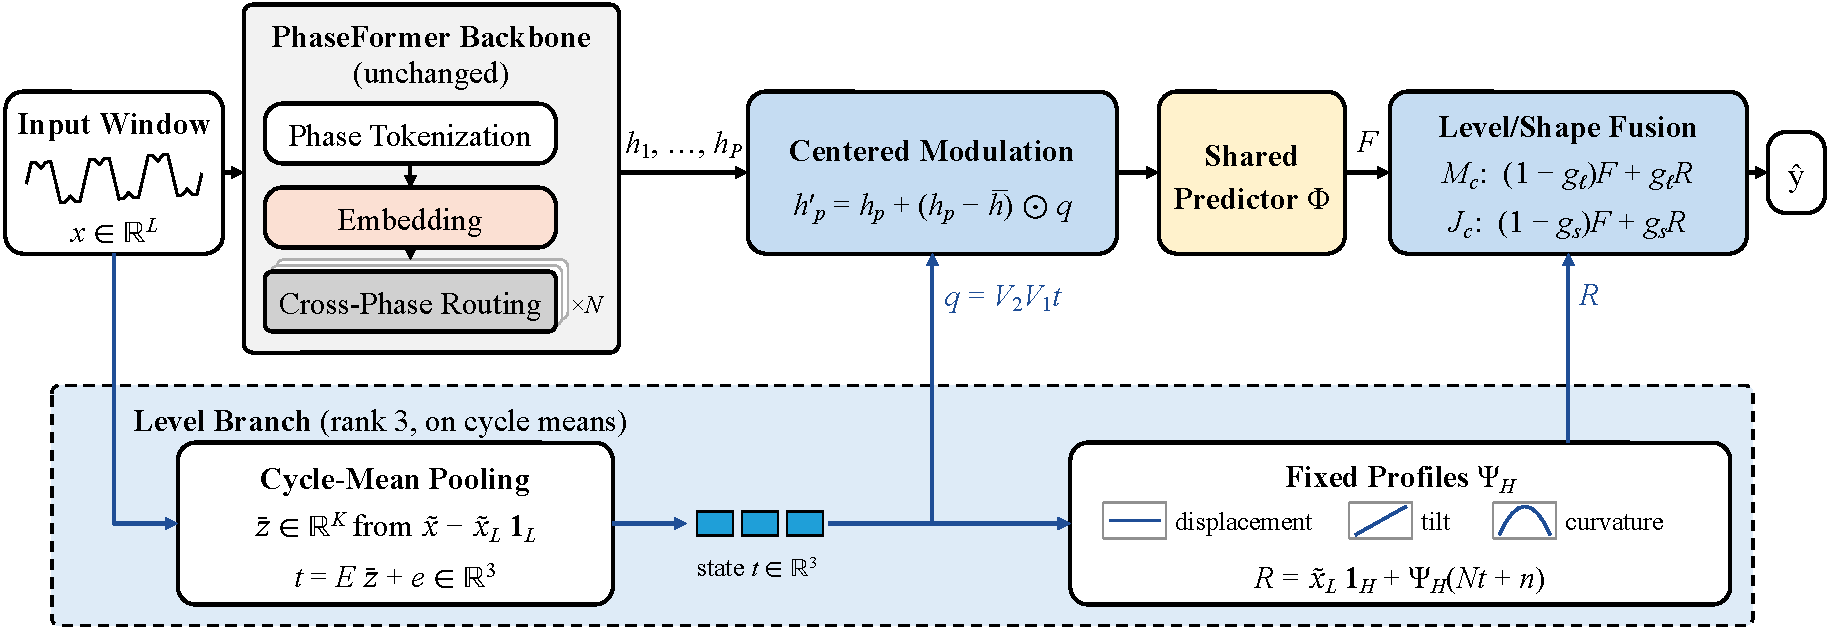
\includegraphics[width=\textwidth]{figures/la_overview.pdf}
\caption{\sysLA. The \sysname backbone and the shared predictor are unchanged and keep the colors of Fig.~\ref{fig:overview}; the new components are blue. A rank-3 level branch reads the anchored cycle means and writes onto three fixed horizon profiles; its state $t$ drives a centered modulation of the final phase latents; the two forecasts are fused with separate level and shape gates.}
\label{fig:la_overview}
\end{figure*}

\fakeparagraph{Notation}
In addition to the notation of Section~\ref{subsec:phase-embedding}, let $\tilde x_L$ be the last value of the normalized window. Let $M_c$ be the orthogonal projection of $\mathbb R^H$ onto the vectors that are constant within each future cycle, and $J_c=I-M_c$: $M_c$ replaces every future cycle by its mean, the level of that cycle, and $J_c$ keeps the deviations within each cycle, its shape. Finally, $\lev(v)=\tfrac1H\one^\top v$ is the level of a forecast $v\in\mathbb R^H$.

\subsubsection{Level Branch and Gated Fusion}
\label{sec:ext_branch}

Level drift adds the same vector of cycle levels to every phase token~\equref{eq:cycle_axis_changes}, so the level of a window is carried by its cycle means, and the level of the future is smooth over the horizon. The branch therefore reads only the cycle means and writes onto a few smooth profiles (left of Fig.~\ref{fig:la_overview}). It pools the anchored window $\tilde x-\tilde x_L\one_L$ to its cycle means $\bar r-\tilde x_L\one_K$ and maps them to a rank-3 state,
\begin{equation}
\begin{gathered}
t=E(\bar r-\tilde x_L\one_K)+c_E\in\mathbb R^3,\\
F_{\mathrm b}=\tilde x_L\one_H+\Psi_H\,(\Gamma t+c_\Gamma),
\end{gathered}
\label{eq:branch}
\end{equation}
where $\Psi_H=[\one_H,a_2,a_3]\in\mathbb R^{H\times3}$ holds the displacement, tilt and curvature profiles, the discrete orthogonal polynomials of degree $0,1,2$ on the forecast grid, normalized to unit root mean square, so that its first column is $\one_H$ and the other two are horizon-centered. $\Psi_H$ is fixed; only $E\in\mathbb R^{3\times K}$, $c_E\in\mathbb R^3$, $\Gamma\in\mathbb R^{3\times3}$ and $c_\Gamma\in\mathbb R^3$ are learned. Theorem~\ref{thm:complement} explains why a map of low rank onto fixed profiles is enough; the main-table configuration replaces $\Psi_H$ by a learned decoder of the same rank on four settings (Appendix~\ref{app:la_config}). The anchor makes the branch shift-equivariant in normalized coordinates: adding $c\one_L$ to $\tilde x$ leaves $t$ unchanged and adds $c\one_H$ to $F_{\mathrm b}$. The branch reads the window directly and is fused after the shared predictor, so, unlike the phase forecast, it passes through no LayerNorm of the backbone; Section~\ref{sec:theory_level} shows why this matters.

\fakeparagraph{Gated Fusion}
For every future cycle, the fused forecast takes its level and its within-cycle shape from $F$ and $F_{\mathrm b}$ with separate gates,
\begin{equation}
\begin{gathered}
M_c\hat{\tilde y}=(1-g_\ell)M_cF+g_\ell M_cF_{\mathrm b},\\
J_c\hat{\tilde y}=(1-g_s)J_cF+g_sJ_cF_{\mathrm b},
\end{gathered}
\label{eq:fusion}
\end{equation}
with $g_\ell=\operatorname{sigmoid}(\omega)$ and $g_s=\operatorname{sigmoid}(\omega+\delta)$. Since $J_c\one_H=0$, the branch enters the within-cycle shape only through the within-cycle parts $J_ca_2$ and $J_ca_3$ of its tilt and curvature profiles. The gates are static: they depend on neither the input nor the time step. They are learned either per channel or shared across the $C$ channels, a choice made per dataset in the protocol configuration and per setting in the main-table configuration (Section~\ref{sec:ext_setup} and Appendix~\ref{app:la_config}).

\subsubsection{Centered Amplitude Modulation}
\label{sec:ext_modulation}

Level-dependent amplitude scales the cycle shape with the level. Before the shared predictor, \sysLA scales the deviations of the final phase latents $h_1,\dots,h_P$ from their mean over the phases, elementwise, by a vector $q$ computed from the branch state $t$, which carries the level forecast (center of Fig.~\ref{fig:la_overview}):
\begin{equation}
h'_p=h_p+(h_p-\bar h)\odot q,\qquad \bar h=\tfrac1P\textstyle\sum_ph_p,\qquad q=V_2V_1\,t,
\label{eq:la_modulation}
\end{equation}
with $V_1\in\mathbb R^{k_q\times3}$, $V_2\in\mathbb R^{d\times k_q}$, $k_q=\min(w,3,d)$ and no biases; the width $w$ is $2$ by default, and the branch rank caps $k_q$ at $3$. The predictor then receives $h'_p$ in place of $h_p$. Because the predictor~\equref{eq:predictor} is shared and affine, $\Phi\bar h+c_\Phi$ is the vector of future cycle means of the phase forecast: $\bar h$ is the latent counterpart of the cycle level, and $h_p-\bar h$ that of the within-cycle shape. The deviations sum to zero over the phases, so the modulation leaves every future cycle mean of the phase forecast unchanged (Proposition~\ref{prop:modulation}(a)): it changes only the within-cycle part of the phase forecast, never its cycle means, and $q=q_1\one_d$ scales that part by $1+q_1$. This centering is over the phases, not over the features as in a LayerNorm.

\subsubsection{Nesting and Initialization}
\label{sec:ext_properties}

The new parameters are initialized so that the components start from simple forecasts. $\Gamma$ and $c_\Gamma$ are zero, so the branch initially forecasts the last value; $V_2$ is zero, so the modulation is initially the identity; and both gates start at a common value $g_0$ ($\delta=0$), $0.2$ by default. With $V_2=0$, \sysLA reduces exactly to \sysL, and \sysL tends to \sysname as $g_\ell,g_s\to0$. Hence \sysLA and \sysL built from the same random state with the same gate initialization have identical forecasts at initialization, which our experiments use to pair them. We write \sysLA (mod.\ off) for a trained \sysLA evaluated with $V_2=0$.
}

\subsection{Complexity of \sysname{} \blue{and \sysLA}}
\label{sec:complexity}

For each \blue{channel}, the overall complexity of \sysname\ can be summarized as follows:
the phase embedding layer requires $O(L_{\text{phase}} P_{\text{in}} d)$ time and $O(L_{\text{phase}} d)$ memory.
The cross-phase routing layer, which dominates computation, incurs $O((L_{\text{phase}}+M)d^2 + M L_{\text{phase}} d)$ time and $O(\blue{n_h} M L_{\text{phase}} + (L_{\text{phase}}+M)d)$ memory.
Finally, the predictor costs $O(L_{\text{phase}} d P_{\text{out}})$ time and $O(L_{\text{phase}} P_{\text{out}})$ memory.
Aggregating across \(\blue{N_r}\) \blue{routing layers and substituting} $P_{\text{in}}=\lceil L_{\text{in}}/L_{\text{phase}}\rceil$ and
$P_{\text{out}}=\lceil L_{\text{out}}/L_{\text{phase}}\rceil$\blue{, the end-to-end time complexity is}
\[
O\Big(\blue{N_r}\big((L_{\text{phase}}+M)d^2 + M L_{\text{phase}} d\big)
+ d(L_{\text{in}}+L_{\text{out}})\Big).
\]
As investigated in \secref{sec:mot_stability}, the phase token space exhibits \blue{an} inherently low-dimensional structure, which allows $M$ and $d$ to be chosen as fixed and small numbers.
Thus, \blue{for a fixed number of layers,} the computational cost grows \blue{linearly} with both the input length $L_{\text{in}}$ and the output horizon $L_{\text{out}}$.

\blue{
\fakeparagraph{Cost of \sysLA}
The level branch adds $3K$ ($E$) $+\,3$ ($c_E$) $+\,9$ ($\Gamma$) $+\,3$ ($c_\Gamma$) $=105$ parameters at $K=30$ with the fixed profiles of \equref{eq:branch}, the modulation $k_q(3+d)$, and the gates $2C$ for $C$ channels, or two in total when shared; none of these depends on the forecast horizon. The branch costs $O(L)$ per channel for pooling and $O(K+H)$ for the readout, and the modulation $O(Pd)$, against the $O\big(N_r((P+M)d^2+MPd)+d(L+H)\big)$ of \sysname, so the overall complexity remains linear in the input and output lengths and in the number of channels.
}
